\section{Implementação.}
As três classes principais da implementação da Meta-heurística de Colônia de Formigas são apresentadas
na Figura \ref{fig:modelo_aep}.

\begin{figure}[ht]
  \centering
  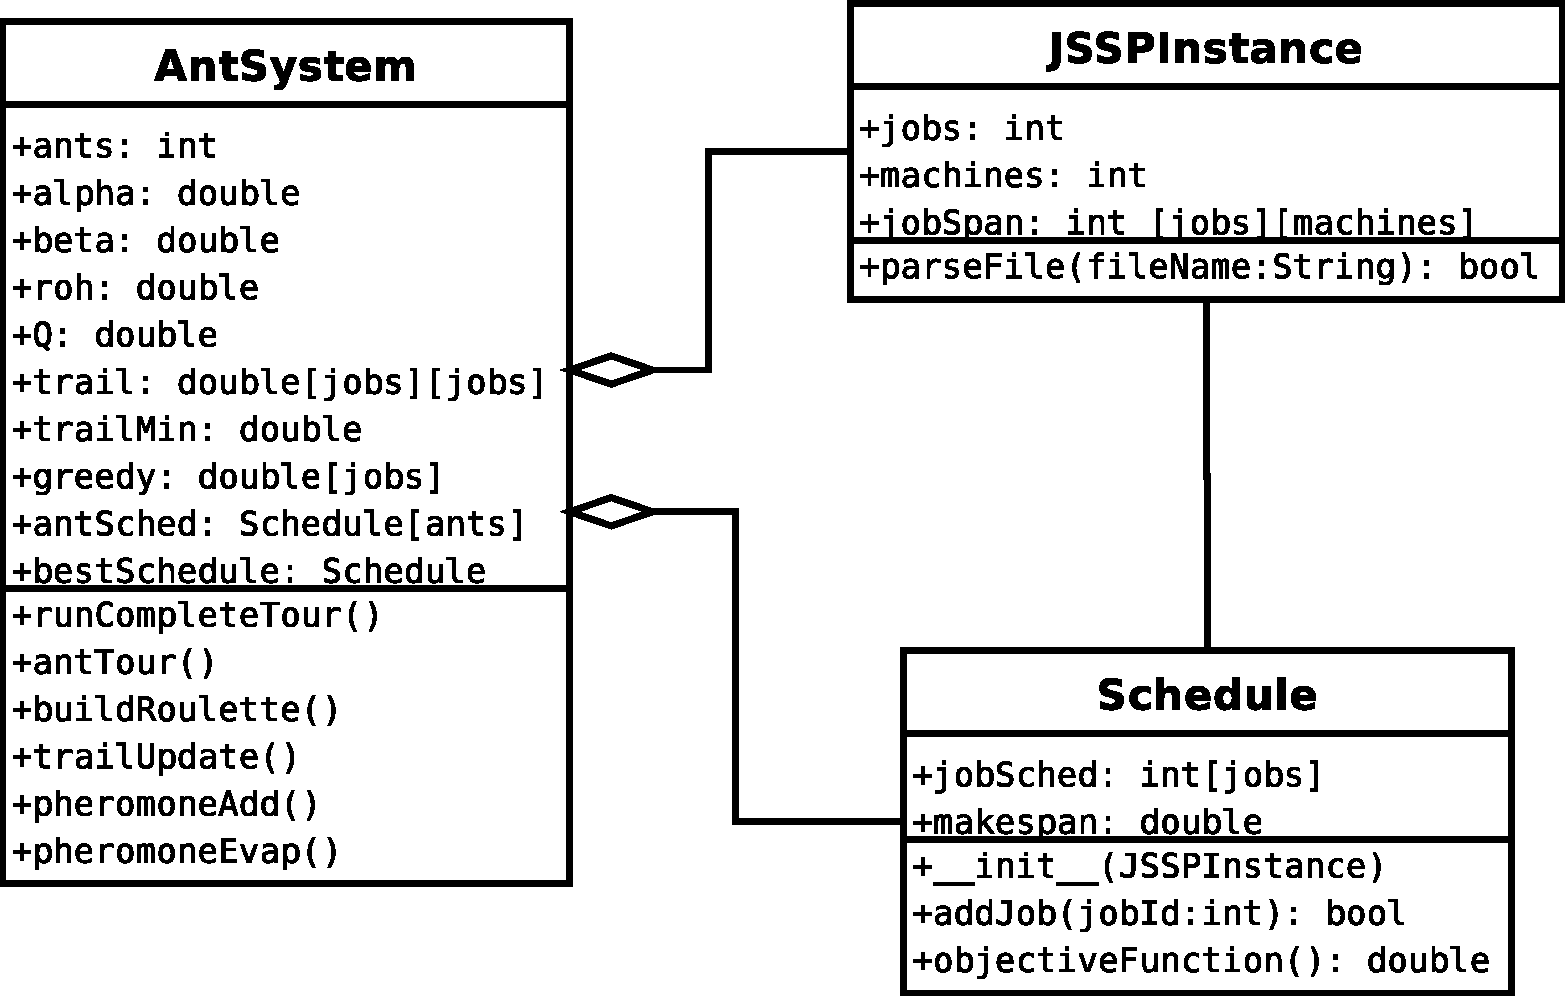
\includegraphics[scale=0.4]{./fig/modelo_aep.pdf}
  \caption{Principais classes da implementação.}
  \label{fig:modelo_aep}
\end{figure}

O núcleo da implementação está na classe AntSystem, que contém todo o código associado a Meta-heurística
de Colônia de Formigas.
A classe JSSPInstance é a responável por ler o arquivo com a instância do problema. A classe Schedule
contém uma sequência de tarefas que formam uma solução válida, ela também é responsável por calcular
o \textit{makespan} associado a sua solução.


\subsection{Customizações.}
Algumas mudanças foram introduzidas nesta implementação, a fim de melhorar seu desempenho,
tornando-a ligeiramente diferente da proposta original \cite{colorni1994ant}.

Uma das mudanças foi na função que adiciona feromônio às rotas percorridas pelas formigas. A implementação
original, também conhecida como elitista, adiciona feromônio a todos os arcos percorridos pelas formigas em 
uma iteração de forma proporcional a qualidade da solução obtida. Contudo, verificou-se que um número elevado
de iterações é necessário para que o nível de feromônio em uma rota se destaque dos demais. Para acelerar este 
processo, adicionamos feromônio apenas nos arcos que compõem a melhor solução da iteração. Ou seja, se existirem
dez formigas decobrindo dez rotas por iteração, apenas uma delas, a melhor, receberá feromônio.

Um ponto sem consenso em \cite{colorni1994ant} e \cite{Zwaan99antcolony} é o valor de inicialização de feromônio.
Adotou-se a estratégia de inicializá-los com o inverso do somatório dos tempos totais de cada tarefa, ver \eqref{eq:trail_min}.
Desta forma, inicializa-se cada arco o valor de feromônio relativo a pior solução possível, solução onde as tarefas são executadas
sequencialmente sem paralelismo.

\begin{equation} \label{eq:trail_min}
Feromonio_{ini,min} = \frac{1}{\sum_{j=1}^{jobs}\sum_{m=1}^{maqs}t_{jm}}
\end{equation}

A proposta original \cite{colorni1994ant} não utiliza um valor mínimo de feromônio em um arco. Assim, com o avançar das 
iterações o nível de feromônio em um arco pode chegar muito próximo de zero, praticamente anulando a probabilidade do arco 
ser selecionado. Utiliza-se o valor em \eqref{eq:trail_min} como valor mínimo para manter a um probabilidade baixa, mas não
nula, do arco ser selecionado.

Em \cite{colorni1994ant}, no início de cada iteração as formigas são colocadas em um job(nó) artificial e a partir daí elas 
selecionam qual job irá ocupar a primeira posição de seu \textit{schedule}. Utilizou-se uma estratégia diferente a fim de 
ampliar e intensificar o espaço de busca. Em 70\% das vezes, a posição inicial é definida de forma randômica, no restante 
a formiga inicia na primeira posição da melhor solução. 

